\documentclass[a4paper]{article}

\usepackage{graphicx}
\usepackage{amsmath}
\usepackage[margin=2.5cm]{geometry}

\title{Methods for elimination of crosstalk and inertial effects in bicycle and
motorcycle steer torque estimation}

\author{Jason K. Moore and Mont Hubbard}

\date{September 30, 2013}

\begin{document}

\maketitle

\section*{Introduction}

To control a bicycle or motorcycle, the rider's primary means of directing the
vehicle is to apply forces to the handlebars which cause the front frame to
rotate relative to the rear frame. The rider can, of course, also use other
more subtle biomechanical motions to influence motion of vehicles, especially
lighter-weight ones, but it is known that forces applied to the handlebar give
much more control authority than other means regardless of the vehicle's
inertia \cite{Sharp2007,Sharp2008a}.

From a modeling perspective, it is generally easier to model the interface
forces as a single torque about the steer axis which acts between the front and
rear frames. The rider can be assumed to be part of the rear frame, regardless
of whether rider is assumed to be rigid or not.

Due to this modeling assumption and ease of measurement, most experimental
measurements of the interface forces between the rider and the front frame are
obtained by measuring the torque generated in the steer axis of the front
frame. These direct measurements of rider applied steer torque are susceptible
to error from two major causes: (1) inertia effects of the front frame which
are located between the sensor and the rider's hands and (2) cross talk from
rider applied forces other than those which generate steer torque. Accounting
for the error sources are particularly important when the steer torques are
small ($<$~20 Nm or so).

In this paper we review previous methods of steer torque measurement in
bicycles and motorcycles and detail the design and implementation of a bicycle
steer torque measurement system which minimizes the aforementioned cross talk
errors. We then show the computations needed to correctly compensate for
inertial effects of the front frame and bearing friction to obtain a more
accurate estimate of the rider applied steer torque. Finally, to show the need
for this approach, we compare the differences between uncompensated and
compensated steer torque measurements for a large set of bicycle experiments.

\section*{History of Steer Torque Measurements}

The earliest steer torque measurements were performed in 1951. Wilson-Jones
\cite{Wilson-Jones1951} developed a set of motorcycle handlebars mounted in
rubber bushings that indicated the direction and value of torque in an analog
fashion in real time. He demonstrated that a negative torque is applied with
respect the steering angle to enter into a turn and measured torques in normal
maneuvers in the 4 to 14 Nm range. Not long after this Kondo \cite{Kondo1955}
was the first to record torque measurements on a motorcycle for post-experiment
analysis. Work in Japan on motorcycle dynamics grew considerably after World
War II due to sanctions on aircraft research. Kageyama \cite{Kageyama1959} and
Fu \cite{Fu1965} continued to improve steer torque measurements in motorcycles
and further studied steady turning. Eaton \cite{Eaton1973} was the first to
measure and record motorcycle steer torque in the United States. He attached a
third handle bar above the regular handlebars with strain gages that produced
voltage proportional to the applied torque around the steer axis while the
rider operated the motorcycle with one hand. He measured steer torques up to
3.4 Nm for straight riding for speeds of 15 to 30 mph. This led him to conclude
that most of the steer torque was due to rider remnant, as opposed to
deliberate control. Not long after this, Weir \cite{Weir1979a} developed a
modular torque sensor which could be affixed to multiple motorcycles with a
$\pm$ 70 Nm range and a 1\% accuracy with a 10 Hz bandwidth and was careful to
reduce crosstalk from other forces applied to the handlebars. They
unfortunately oversized the sensor and the signal to noise ratio was low for
steady turn and straight riding maneuvers, but they measured torques of -20 to
55 Nm in lane changes. Sugizaki \cite{Sugizaki1988} also measured steer torque
in high speed motorcycle lane change maneuvers and recorded torques between -20
and 20 Nm.

After years of motorcycle steer torque measurements, the first bicycle
measurements were made by de Lorenzo \cite{Lorenzo1997} on a downhill mountain
bicycle which was fitted with a custom strain gauged handlebar that could
effectively measure torque about the longitudinal axis and the vertical axis.
His plot of torque measurements show maximum steer torques of 7 Nm and maximum
longitudinal handlebar torques of 15 Nm which demonstrated that non-steer
related forces on the handlebars can be significantly higher that those needed
for steering.

Around the turn of the 21st century, Bortoluzzi \cite{Bortoluzzi2000} designed
a successful motorcycle steer torque transducer in which floating handlebars
engage the fork through a small strain-gaged cantilever beam. This design was
less susceptible to crosstalk than earlier designs. They found torques up to
20 Nm for slalom maneuvers at 40 m/s. Around the same time, James
\cite{James2002} developed a secondary handlebar with integrated load cell to
measure steer torques in an off-road motorcycle.

In 2003, Cheng \cite{Cheng2003} completed a comprehensive study on bicycle
steer torque for an undergraduate project. Cheng started by simply attaching a
torque wrench to a bicycle and made left turns at speeds from 0 to 13 m/s and
found that most steering torques were under 5 Nm. He then designed a floating
handlebar which engaged the steer tube via a linear load cell, configured to
measure torques of 0 to 84 Nm. Cheng found torques up to 1 Nm for steady
turning at 4.5 m/s and up to 10 Nm for sharp turns, confirming that bicycles
require much lower torques for maneuvering.

Iuchi \cite{Iuchi2006} constructed a bicycle with a steer motor that ``senses''
the rider's input for use in additive control. The rider applied steer torque
was estimated from the motor torque and the handlebar and motor moments of
inertia. Capitani \cite{Capitani2006} found measured steer torques from an
instrumented scooter between -15 and 40 Nm. Evertse \cite{Evertse2010} was
perhaps the only person to estimate steer torque from sensors in the handle
grips of a motorcycle that give force measurements directly at the
human-vehicle interface. During the test maneuvers, a maximum of 40 Nm was
observed. In 2010, Teerhuis \cite{Teerhuis2010} shows measured torques just
under 20 Nm for a motorcycle in slalom maneuvers.

Recently, Cain \cite{Cain2012} developed an in-the-steer-tube torque sensor for
a bicycle. The measured steer torques in steady turns never exceed 2.4 Nm but
he admits that his sensor was 90\% oversized. And most recently, van den Ouden
\cite{Ouden2011} developed a steer torque sensor sensor that was susceptible to
cross talk from other handlebar loads but had an appropriate measurement range
of $\pm7.5$ Nm.

Steering torque has been measured in relatively few instances of bicycle
experiments and not many more for motorcycles. Of these, very few of the
designs may actually measure the true rider applied steer torque. This is more
consequential for bicycles than motorcycles because the small torques used in
typical bicycle control are of the order of 5-10 Nm. van den Ouden
\cite{Ouden2011}, in particular, showed how sensitive the torque measurements
are to other handlebar loads. Also, most of these designs measure the torque
somewhere between the rider hands and the ground contact point. This is a
physically ideal way to measure the steer torque, but apparently no one has
accounted for the dynamic inertial effects of the front frame above or below
the sensor, except Iuchi \cite{Iuchi2006}. Evertse \cite{Evertse2010} may
have the only design which mitigates this inertial compensation issue
completely.

With this information in hand we designed a steer torque measurement system for
a bicycle that accounts for the deficiencies in previous designs.

\section*{Isolated Steer Torque Measurement Design}

Our design is based on a Futek 150 in-lb ($\pm 17$ Nm) TFF350 torque sensor to
ensure high accuracy for the low torques used in normal bicycle maneuvering.
To guarantee that torques are measured only about the steer axis we isolated
the steer torque sensor from any of the non-axial torques and all forces
transmitted through the handlebar or ground contact with a zero backlash
telescoping double universal joint, Figure~\ref{fig:steer-torque-design}.

\begin{figure}
  \centering
  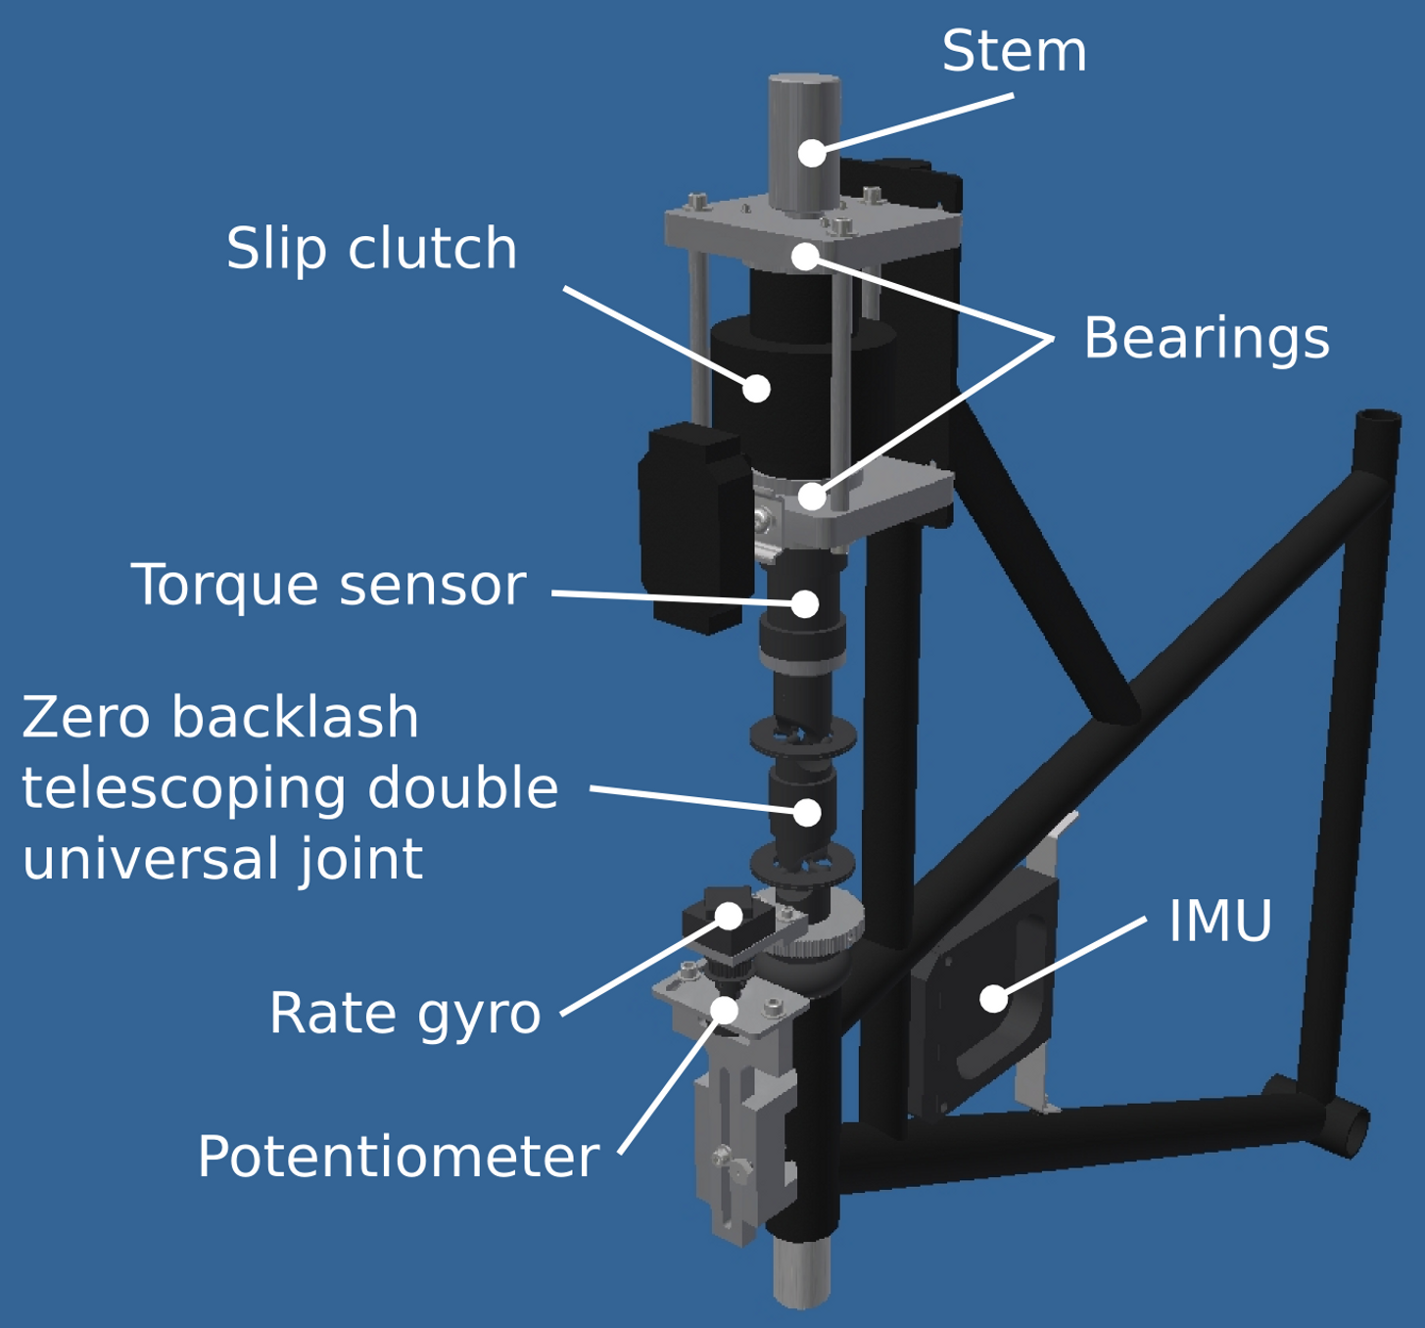
\includegraphics[width=3in]{figures/steer-torque-design.png}
  \caption{The steer torque sensor isolation design. The handlebars attach to
    the stem which is mounted in the upper bearings. The fork and steer tube
    are mounted in the normal headset of the bicycle. Between these two sets of
    bearings the stem is connected to the steer tube via the torque sensor and a
    zero backlash telescoping double universal joint. The steer angle and rate
    are measured at the steer tube and rate and acceleration of the rear frame
    are collected with the IMU.}
  \label{fig:steer-torque-design}
\end{figure}

\section*{Steer Dynamics}
\label{sec:steer-dynamics}

The final design measured the torque in the steer tube along the steer axis,
but this measured torque $T_M$ is not the same as the effective input torque
applied by the rider. The rider applied steer torque $T_\delta$ can be shown to
be a function of the kinematics of the front and rear frame and the friction
torques generated by the bearings.

A free body diagram can be drawn of the portion of the front frame assembly
above the torque sensor, Figure~\ref{fig:handlebar-free-body}. The torques
acting on the handlebar about the steer axis are the measured torque $T_M$ the
rider applied steer torque $T_\delta$ and the friction from the upper bearing
set $T_U$ which we describe by the sum of Coulomb $T_{U_F}$ and viscous
friction $T_{U_V}$.

\begin{figure}
  \centering
  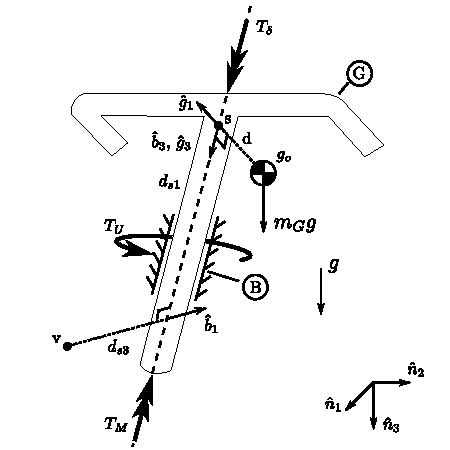
\includegraphics{figures/handlebar-free-body.pdf}
  \caption{A free body diagram of the handlebar, $G$, with all axial torques
    shown. The rear frame $B$ has arbitrary orientation with respect to the
    Newtonian reference frame $N$. The handlebar rotates about $\hat{b}_3$ with
    respect to the rear frame. Gravity $g$ is in the $\hat{n}_3$ direction. The
    rider applies forces to the handlebars, resulting in a component of torque
    $T_\delta$ about the steer axis. This torque is resisted by the upper
    bearing friction $T_U$, the measured torque at the sensor $T_M$, the
    inertia of the handlebar, and the gravitational force acting on the
    handlebar center of mass $g_o$. The three distances, $d$, $d_s1$, and
    $d_s3$ locate the handlebar center of mass with respect to the center of
    the IMU.}
  \label{fig:handlebar-free-body}
\end{figure}

We measure three components of body fixed angular rate of the rear frame $B$ in
the Newtonian reference frame $N$ with three rate gyros. This is written as

\begin{equation} ^N\bar{\omega}^B = w_{b1}\hat{b}_1 + w_{b2}\hat{b}_2 +
  w_{b3}\hat{b}_3
  \label{eq:rear-frame-angular-rate}
\end{equation}

The handlebar $G$ is connected to the bicycle frame $B$ by a revolute joint
that rotates through the steering angle $\delta$ and we measure a component of
the body fixed inertial angular rate of the handlebar $w_{h3}$ about the steer
axis with a rate gyro. The angular velocity of the handlebar can be written as

\begin{equation}
  ^N\bar{\omega}^G = (w_{b1}c_\delta + w_{b2}s_\delta)\hat{g}_1 +
  (-w_{b1}s_\delta + w_{b2}c_\delta)\hat{g}_2 +
  w_{h3}\hat{g}_3
\end{equation}

where $c_\delta$ and $s_\delta$ are shorthand for $\operatorname{cos}(\delta)$
and $\operatorname{sin}(\delta)$ respectively.

The steer rate, $\dot{\delta}$, can be computed by subtracting the angular rate
of the bicycle frame about the steer axis from the angular rate of the
handlebar about the steer axis.

\begin{equation}
  \dot{\delta} = w_{h3} - w_{b3}
\end{equation}

Now we define a point $s$ on the steer axis a minimum distance $d$ from the
center of mass of the handlebar $g_o$.

\begin{equation}
  \bar{r}^{g_o/s} = d\hat{g}_1
\end{equation}

We also measure the body fixed acceleration of a point $v$ on the bicycle frame
which includes the acceleration due to gravity.

\begin{equation}
  ^N\bar{a}^v = a_{v1}\hat{b}_1 + a_{v2}\hat{b}_2 + a_{v3}\hat{b}_3
  \label{eq:acceleration-of-v}
\end{equation}

The location of point $v$ is known with respect to $s$

\begin{equation}
  \bar{r}^{s/v} = d_{s1}\hat{b}_1 + d_{s3}\hat{b}_3
\end{equation}

The acceleration $^N\bar{a}^{g_o}$ can now be calculated using the two point
theorem for acceleration \cite{Kane1985} twice starting at the point $v$

\begin{equation}
  ^N\bar{a}^s = {}^N\bar{a}^v +
    {}^N\dot{\bar{\omega}}^B\times\bar{r}^{s/v} +
    {}^N\bar{\omega}^B\times({}^N\bar{\omega}^B\times\bar{r}^{s/v})
\end{equation}

\begin{equation}
  ^N\bar{a}^{g_o} = {}^N\bar{a}^s +
    {}^N\dot{\bar{\omega}}^G\times\bar{r}^{g_o/s} +
    {}^N\bar{\omega}^G\times({}^N\bar{\omega}^G\times\bar{r}^{g_o/s})
\end{equation}

The angular momentum of the handlebar about its center of mass is

\begin{equation}
  ^N\bar{H}^{G/g_o} = I^{G/g_o} \cdot {}^N\bar{\omega}^G
\end{equation}

where $I^{G/g_o}$ is the inertia dyadic with reference to the center of mass
which exhibits symmetry about the 1-3 plane.

Now the dynamic equations of motion of the handlebar can be written: the sum of
the torques on the handlebar about point $s$ equals the derivative of the
angular momentum of $G$ in $N$ about $g_o$ plus the cross product of the vector
from $s$ to $g_o$ with the mass times the acceleration of $g_o$ in $N$
\cite{Meriam1975}. We neglect the gravitational torque because it is already
accounted for in the measured linear acceleration,
Equation~\ref{eq:acceleration-of-v}.

\begin{equation}
  \sum \bar{T}^{G/s} = {}^N\dot{\bar{H}}^{G/g_o} +
    \bar{r}^{g_o/s} \times m_G\,{}^N\bar{a}^{g_o}
\end{equation}

We are only interested in the components of the previous equation in which the
steer torque appears, so only the torques about the steer axis are examined.

\begin{equation}
  \sum T^{G/s}_3 = T_\delta - T_U - T_M = \left({}^N\dot{\bar{H}}^{G/g_o} +
  \bar{r}^{g_o/s} \times m_G\,{}^N\bar{a}^{g_o}\right) \cdot \hat{g}_3
\end{equation}

Finally, $T_\delta$ can be written as

\begin{align}
  T_{\delta} =
    & I_{G_{22}} \left[ \left( -w_{b1} s_\delta + w_{b2} c_\delta \right)
      c_\delta + w_{b2} s_\delta \right] + I_{G_{33}} \dot{w}_{g3} + \nonumber \\
    & I_{G_{31}} \left[ (-w_{g3} + w_{b3} ) w_{b1} s_\delta +
      (-w_{b3} + w_{g3}) w_{b2} c_\delta +
      s_\delta \dot{w}_{b2} + c_\delta \dot{w}_{b1} \right] + \nonumber \\
    & \left[ I_{G_{11}} (w_{b1} c_\delta + w_{b2}s_\delta) +
      I_{G_{31}} w_{g3} \right] \left[-w_{b1} s_\delta +
      w_{b2} c_\delta \right] + \nonumber \\
    & d m_G \left[ d (-w_{b1} s_\delta + w_{b2} c_\delta)
      (w_{b1} c_\delta + w_{b2} s_\delta) + d \dot{w}_{g3} \right] - \nonumber \\
    & d m_G \left[-d_{s1} w_{b2}^{2} + d_{s3} \dot{w}_{b2} -
      (d_{s1} w_{b3} - d_{s3} w_{b1}) w_{b3} + a_{v1} \right] s_\delta + \nonumber \\
    & d m_G \left[d_{s1} w_{b1} w_{b2} + d_{s1} \dot{w}_{b3} +
      d_{s3} w_{b2} w_{b3} - d_{s3} \dot{w}_{b1} + a_{v2} \right]
      c_\delta + \nonumber \\
    & T_U + T_M
\end{align}

All time varying terms in $T_\delta$ are measured by on-board sensors or can be
calculated with numerical differentiation except for the upper bearing
frictional torque, $T_U$. We estimate this torque contribution through
experiments described in the following section. The distance, mass, and inertia
values are measured as described in \cite{Moore2012}.

\section*{Estimation of Bearing Friction}
\label{sec:bearing-friction}

In our design, the torque sensor is mounted between two sets of bearings. The
upper set for the handlebars are tapered roller bearings and the lower are
typical bicycle headset bearings. Each are preloaded a nominal amount during
installation. We assume that the rotary friction due to each bearing set can be
described as the sum of viscous $T_{Bv}$ and Coulomb friction $T_{Bc}$. The
Coulomb friction can be described as a piecewise-constant function of the
steering rate, Equation~\ref{eq:coulomb}, and viscous friction as linear in the
steer rate, Equation~\ref{eq:viscous}.

\begin{equation}
  T_{Bc} = t_B \operatorname{sgn}(\dot\delta) =
  \begin{cases}
    t_B  & \textrm{if $\dot{\delta}>0$}\\
    0    & \textrm{if $\dot{\delta}=0$}\\
    -t_B & \textrm{if $\dot{\delta}<0$}
  \end{cases}
  \label{eq:coulomb}
\end{equation}

\begin{equation}
  \label{eq:viscous}
  T_{Bv} = c_B \dot{\delta}
\end{equation}

The total friction due to all of the bearings is

\begin{equation}
  T_B = T_{Bc} + T_{Bv}
\end{equation}

To estimate the coefficients $t_B$ and $c_B$, we mounted the bicycle with the
steer axis vertical, the front wheel off the ground, and the rear frame rigidly
fixed in inertial space. We then attached two parallel springs of stiffness $k$
to the left handlebar so that the force from the springs acted through lever
arm $l$ relative to the steer axis.

This configuration allowed application of small perturbations to the handlebars
and subsequent measurement of the damped vibrations in the steer angle, steer
rate, and steer tube torque. The equations of motion governing the system then
become

\begin{equation}
  I_{HF} \ddot{\delta} + c_B \dot{\delta} + t_B
  \operatorname{sgn}(\dot{\delta}) + 2 k l^2 \delta = 0
\end{equation}

We measured the lever arm and spring stiffness as 0.213 meters and $904.7 \pm
0.6$ N/m respectively. The inertia of the handlebar, fork, and front wheel
about the steer axis, $I_{HF}$, was estimated based on the measurements
described in \cite{Moore2012} and found to be $0.1297+/-0.0005$ $kg\cdot m^2$

We estimated the friction coefficients with a non-linear grey box
identification based on the measured steer angle over 15 trials in which the
steering assembly was perturbed from equilibrium. The identified viscous
coefficient is $c_B = 0.34 \pm 0.04$ $N \cdot m \cdot s^2$ and the Coulomb
coefficient is $t_B = 0.15 \pm 0.05$ $N \cdot m$.

To calculate the applied steer torque $T_\delta$ we need an estimate of the
upper bearing friction $T_U$. We made the simple assumption that the friction
in the upper and lower bearings are equal, $T_U = T_B / 2$, due to
indeterminacy of the upper and lower bearing friction individually; see
\cite{Moore2012} for details.

\begin{figure}
  \centering
  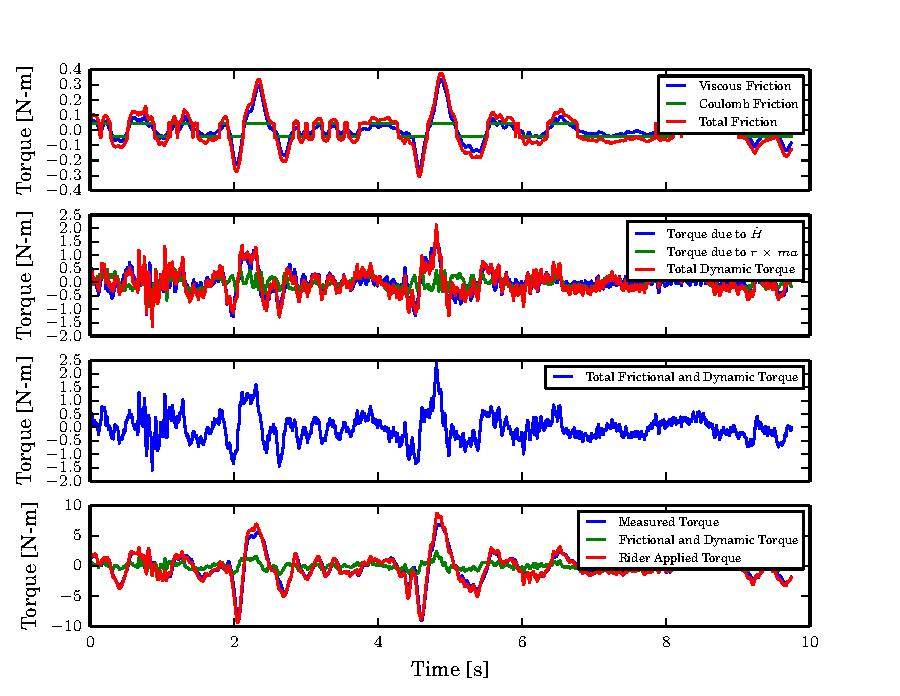
\includegraphics{figures/steer-torque-components.pdf}
  \caption{Steer torque measurements and the computed compensation for Trial \#
    700.}
  \label{fig:steer-torque-components}
\end{figure}

\section*{Steer Torque Predictions}

\begin{figure}
  \centering
  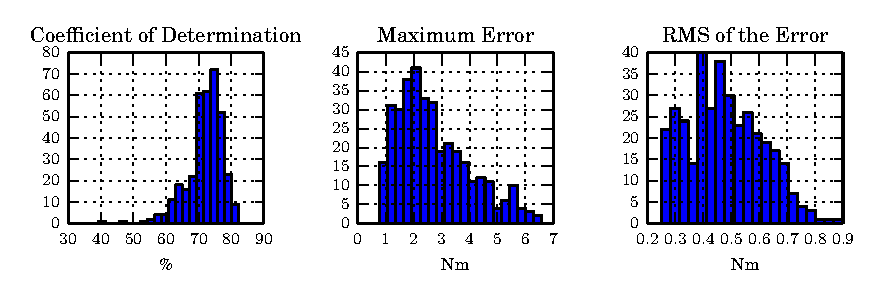
\includegraphics{figures/error-stats.pdf}
  \caption{Histograms of the three statistics for all 359 trials.}
  \label{fig:error-stats}
\end{figure}

Using the equations described in section \ref{sec:steer-dynamics} and the
estimates for the upper bearing friction in \ref{sec:bearing-friction} we
compute the compensated steer torque for 359 trials from the data collected
from the instrumented bicycle set presented in \cite{Moore2012}.
Figure~\ref{fig:steer-torque-components} gives results from an example trial.
We then compute the root mean square of the error between the torque from the
sensor and the compensated torque for each trial. We also compute the maximum
of the absolute value of the error for each trial and the coefficient of
determination (i.e. $R^2$) between the compensated and uncompensated torques.
Outliers outside of $\pm2 \sigma$ were excluded from the results. Figure
\ref{fig:error-stats} shows the distribution of these statistics. The median
values of the three statistics are given in Table~\ref{tab:medians}.

\begin{table}
  \caption{The median and maximum value of the error statistics.}
  \centering
  \begin{tabular}{lrr}
    \hline
    Statistic                    & Median   & Maximum \\
    \hline
    Coefficient of Determination & 0.728814 & 0.822647 \\
    Maximum Error                & 2.446387 & 6.588228 \\
    RMS of the Errors            & 0.466733 & 0.899118
  \end{tabular}
  \label{tab:medians}
\end{table}

\section*{Discussion}

For the bicycle and maneuvers performed in the experiments herein we have shown
that neglecting to compensate for inertial effects can have a large influence
on the accuracy of the results. In particular, on median 28\% of the actual
torque applied by the rider in our experiments would be neglected. This may be
less important for motorcycles because the nominal steer torques are usually
much larger, but this error will always be significant for measurements of low
torque ($<$ 20 Nm or so) in any vehicle. Steer torque sensor designs should
account for the inertial effects of the handlebars and eliminate crosstalk for
high accuracy. Ideally, one would measure the forces at the hand/handlebar
interface with very accurate six component load cells and inertial compensation
would not be necessary. The closer the sensor is to the rider's hands the less
important inertial compensation becomes. But if more traditional direct steer
torque measurements are used, both inertial compensation and cross talk
mitigation (mechanically or computationally) will be needed. We have found only
a couple of designs that mitigate the inertial issue before us, namely
\cite{Evertse2010} and \cite{Iuchi2006}, and many previous design were aware of
crosstalk, but no design shows complete elimination as we have. Maneuvers with
high steer accelerations and high handlebar axial moments of inertia are
especially susceptible, due to the dominance of the effects of angular
acceleration on torque. This is clearly shown in
Figure~\ref{fig:steer-torque-components}. Our design gave very accurate torque
measurements, but there is still much room for improvement, especially in terms
of complexity and cost. Creating a simple, inexpensive, and accurate steer
torque measurement system could play an important role in assistive control
system design in production vehicles.

\section*{Acknowledgements}

This paper is based on work supported by the National Science Foundation under
Grant No. 0928339. Thanks to Peter de Lange for developing the bearing friction
experimental protocol and analysis and to Ton van den Bogert for comments and
review.

\bibliographystyle{plain}
\bibliography{references}

\end{document}
